 Deep Learning is part of machine learning methods based on artificial neural networks. %with representation learning. %Learning can be supervised, semi-supervised or unsupervised. 
 Part of the theoretical basis underlying Deep Learning  initially emerged as models for understanding the human learning process, that is, how the brain works. Thus, these theories are related with Deep Learning  that has grown the most in recent years \cite{goodfellow2016}. Deep learning methods have achieved excellent performance over traditional machine learning methods, mainly due to the development of the area, but also by the increase in computational power and the amount of available data \cite{geron2019}. 

One of the most well known applications of Deep Learning are computer vision problems. Therefore, different from other chapters that discuss potential applications at the end of the chapter, this whole chapter will focus mainly on deep learning for computer vision problems. Computer vision is a field that seeks to reproduce some of the human capabilities through autonomous systems. The main aim of computer vision is to enable computers to perform functions similar to human vision, being able to receive visual data and perform its processing. Examples of computer vision problems include face recognition and object recognition. This field has been using Artificial Intelligence (AI) extensively. The performance improvements in computer vision are strongly related with the evolution of the field of machine learning.

Traditional computer vision techniques were almost entirely pipelined by hand, where the features to be used as input variables were obtained through manually designed methods. This made such techniques more difficult to adapt to different tasks. With the emergence of deep learning, it became possible to use neural networks to automatically learn features to be used. This has helped Deep Learning to outperform other existing methods on several problems such as computer vision problems.

%\begin{figure}
%    \centering
%    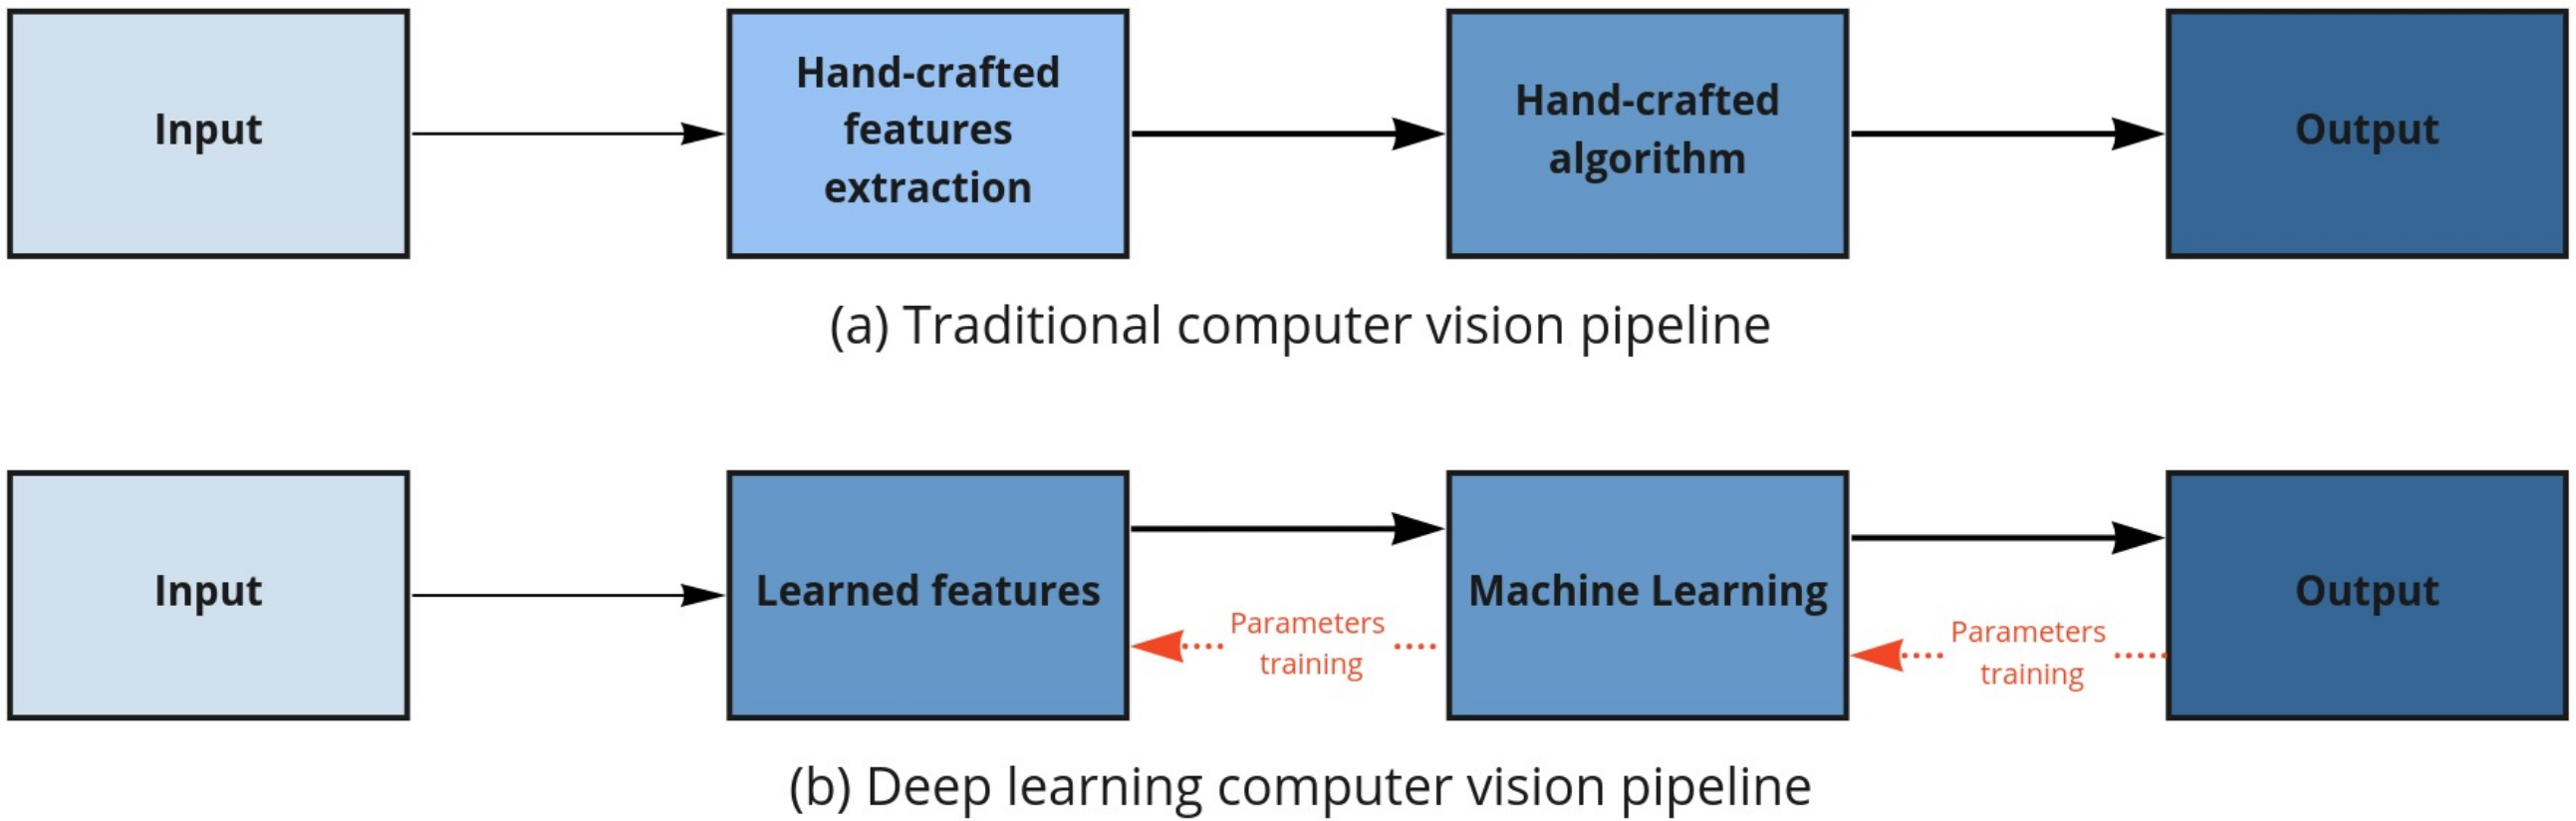
\includegraphics[scale=0.20]{"Part 3 - Learning Systems/Supervised Learning/Deep Learning/images/cvpipeline.png"}
%    \caption{Traditional(a) and Deep learnign(b) computer vision pipelines. Inspired in \cite{szeliski2010computer}(Figure 5.2)}
%    \label{fig:figurecvpipeline}
%\end{figure}
%
%Figure \ref{fig:figurecvpipeline} presents two preprocessing scenarios. The traditional(\ref{fig:figurecvpipeline} (a)), where the two principal steps, the selection of features to be extracted and the algorithm that uses these features, are mannually adjusted. The Deep learning pipeline(\ref{fig:figurecvpipeline} (b)), where the model learns which features to extract and how use these features to get the desired output. The red arrow in the Deep Learning pipeline shows how this type of model uses information about the output to adjust the parameters of the network, and consequently, learns a problem.

Among the many deep learning architectures, the Convolutional Neural Networks (CNN) is one of the most widely used as it is very similar to a conventional Multilayer Perceptron (MLP) introduced in a previous chapter of this book.

\section{Convolutional Neural Networks (CNN)}

As with the MLPs, CNNs are also formed by neurons and connections between them to build a model. Backpropagation is also frequently used to learn the weights of the connections (parameters). However, instead of connecting all neurons of a given layer to all neurons of the previous layer like the MLPs, CNNs has some layers connecting a neuron to a limited number of neurons of the previous layer \cite{Patel2018}. This helps to reduce the amount of memory and computations required by the CNNs. Moreover, instead of using a separate weight to each connection between neurons, some layers of the CNNs share the same matrix of weights for the incoming connections of all neurons of the same layer \cite{Patel2018}. This also helps to reduce the amount of required memory to store the model. Each of such matrices is referred to as a \textit{kernel} or \textit{filter}. 

The next subsections explain the types of layer that are used to compose the CNN, namely convolution, pooling and fully connected layers. There are different possible architectures (ways to arrange layers) for CNNs, where different numbers of each type of layer may be used. Typically, the first layer is a convolution layer, which may be followed by other convolution layers or by pooling layers. The last layers are typically fully connected layers, which are similar to the MLP layers. An example of this is shown in Figure \ref{fig:figure123}. Different examples of CNN architectures are given in Section \ref{sec:architectures}.

\begin{figure}
    \centering
    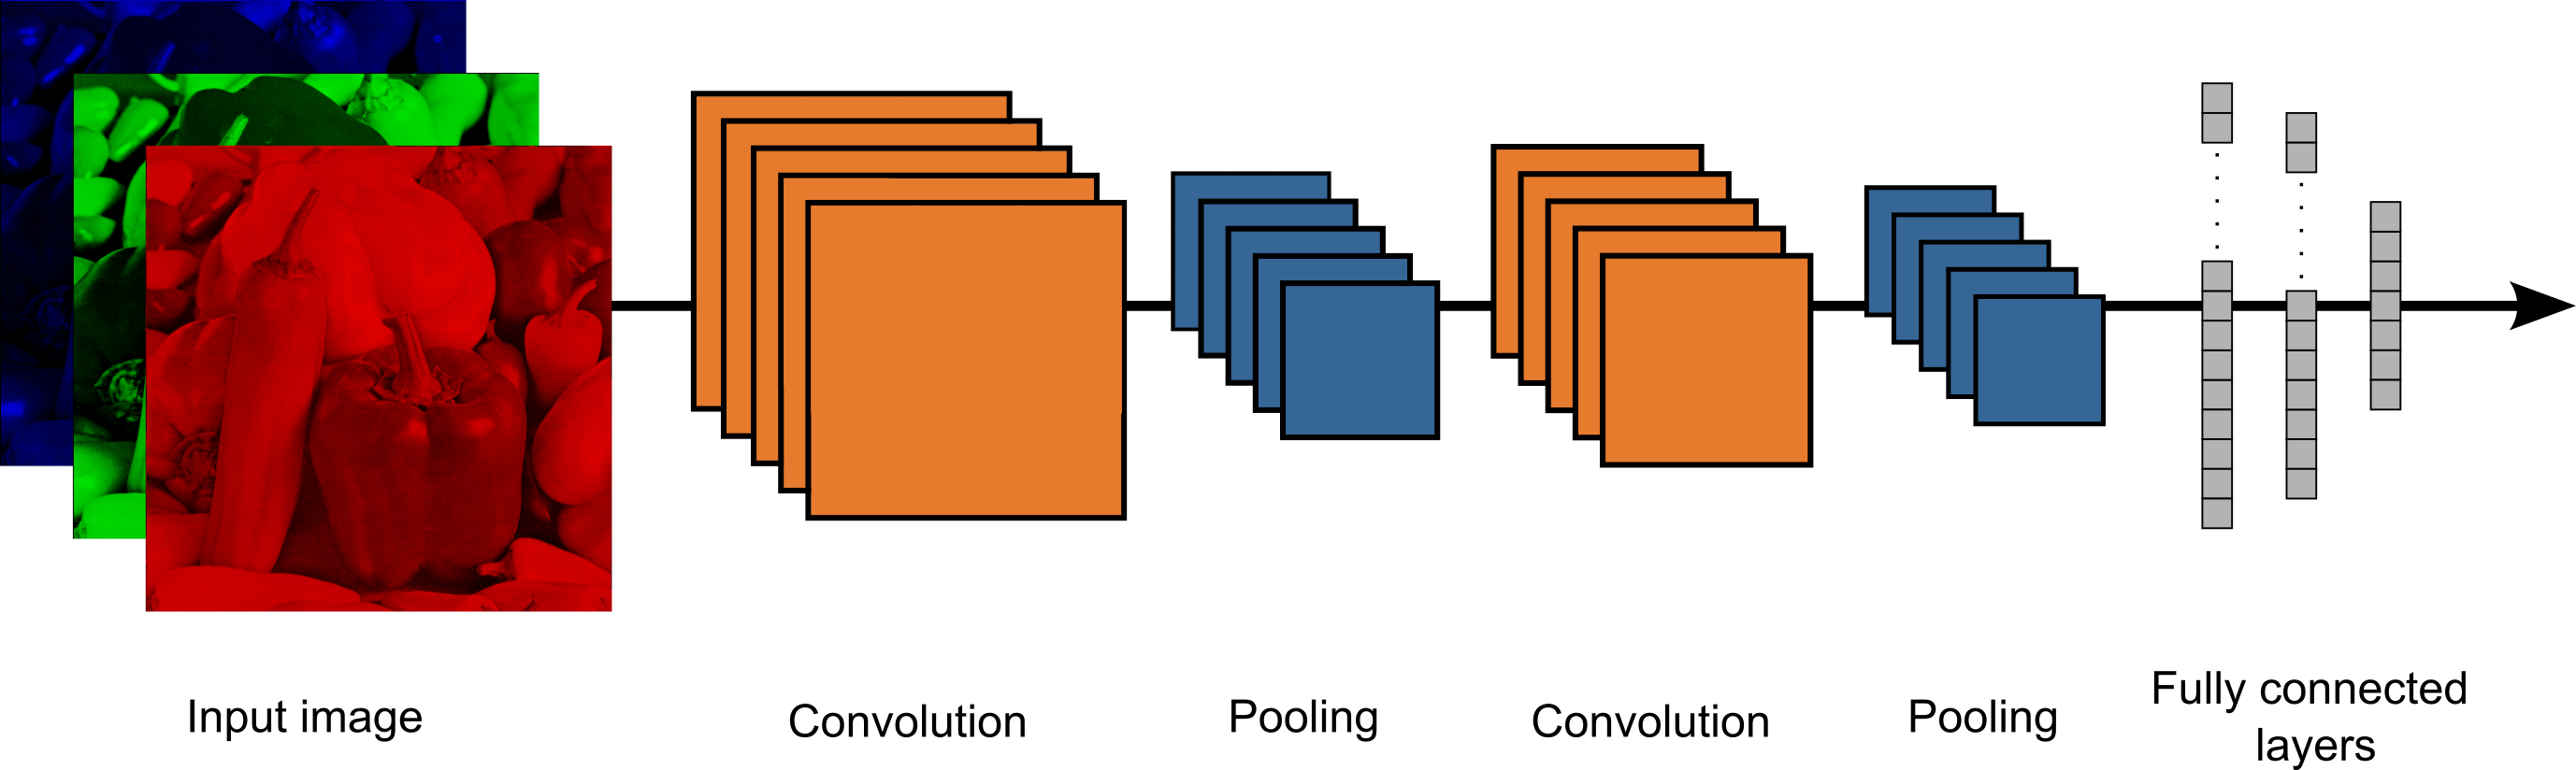
\includegraphics[scale=0.22]{"Part 3 - Learning Systems/Supervised Learning/Deep Learning/images/figure123.png"}
    \caption{Example of CNN architecture.}
    \label{fig:figure123}
\end{figure}

\subsection{Convolution Layers}

The operation that gives name to this artificial neural network is the convolution, which is performed in the convolution layers. This operation systematically applies the kernel to an input image to generate a processed output image. Layers that perform the convolution operation are referred to as convolution layers. The processed image produced by a convolution layer can be seen as summarising the presence of features automatically detected in the input image \cite{Brownlee2019} and is commonly referred to as a feature map. %is an operation performed between two functions. In the case, as the operation is performed with images, discrete convolution is used.

%An important point to note is that mathematically what we will call a convolution is actually a correlation, and the two are almost identical, except for the fact that in the convolution we rotate the filter (kernel) by 180\textdegree . The only advantage we gain from turning the filter before the operation is that we gain the commutative property, which is mathematically useful for proof derivation but not important in Deep Learning  implementation \cite{goodfellow2016}.

In Deep Learning  literature and libraries, it has become common to call this operation as convolution \cite{goodfellow2016}, though mathematically this operation is known as  correlation. The convolution operation $g(x,y)$ applied to a pixel with coordinates $(x,y)$ is defined in Equation \ref{correlation}:

\begin{equation}
\label{correlation}
g(x,y)= \sum_{s=-a}^a\sum_{t=-b}^bW_{s,t}F_{x+s,y+t}
\end{equation}

\noindent where $W$ is a kernel, which is a matrix of numbers, usually with odd square size $2a + 1$ by $2b + 1$ (to facilitate operations); $a$ and $b$ are pre-defined values to define the size of the kernel and determine the possible values of its coordinates; and $F$ represents an image in matrix format. For convenience, the first coordinate of the matrix $F$ is set as $(-a,-b)$. %And related to this is the formula of convolution ($g$):

%\begin{equation}
%g(x,y)=w(x,y)\ast f(x,y)=\sum_{s=-a}^a\sum_{t=-b}^bw(s,t)f(x-s,y-t)
%\end{equation}

Figure \ref{fig:figure117} presents an example of correlation step taking place. In this figure, $a=b=1$, and the indices of the elements of the matrices start with -1 instead of starting with 1. For instance, the coordinate $x$ of the matrix $F$ goes from -1 to 3. The convolution operation is being applied to pixel $F_{0,0}$. The operations performed in this convolution step are:

%corrigir orientação
\begin{equation}
\begin{split}
g(0,0)=\sum_{s=1}^{2}\sum_{t=1}^{2}W_{s,t}{F}_{0+s,0+t}= \\
w(-1,-1)f(-1,-1)+w(-1,0)f(-1,0)+w(-1,1)f(-1,1) \\
+w(0,-1)f(0,-1)+w(0,0)f(0,0)+w(0,1)f(0,1) \\
+w(1,-1)f(1,-1)+w(1,0)f(1,0)+w(1,1)f(1,1)\\
=(-1)\cdot5+(-2)\cdot7+(-1)\cdot0\\
+0\cdot6+0\cdot0+0\cdot1\\
+1\cdot6+2\cdot2+1\cdot2
=-19-0+12=-7
\end{split}
\end{equation}

\begin{figure}[h]
    \centering
    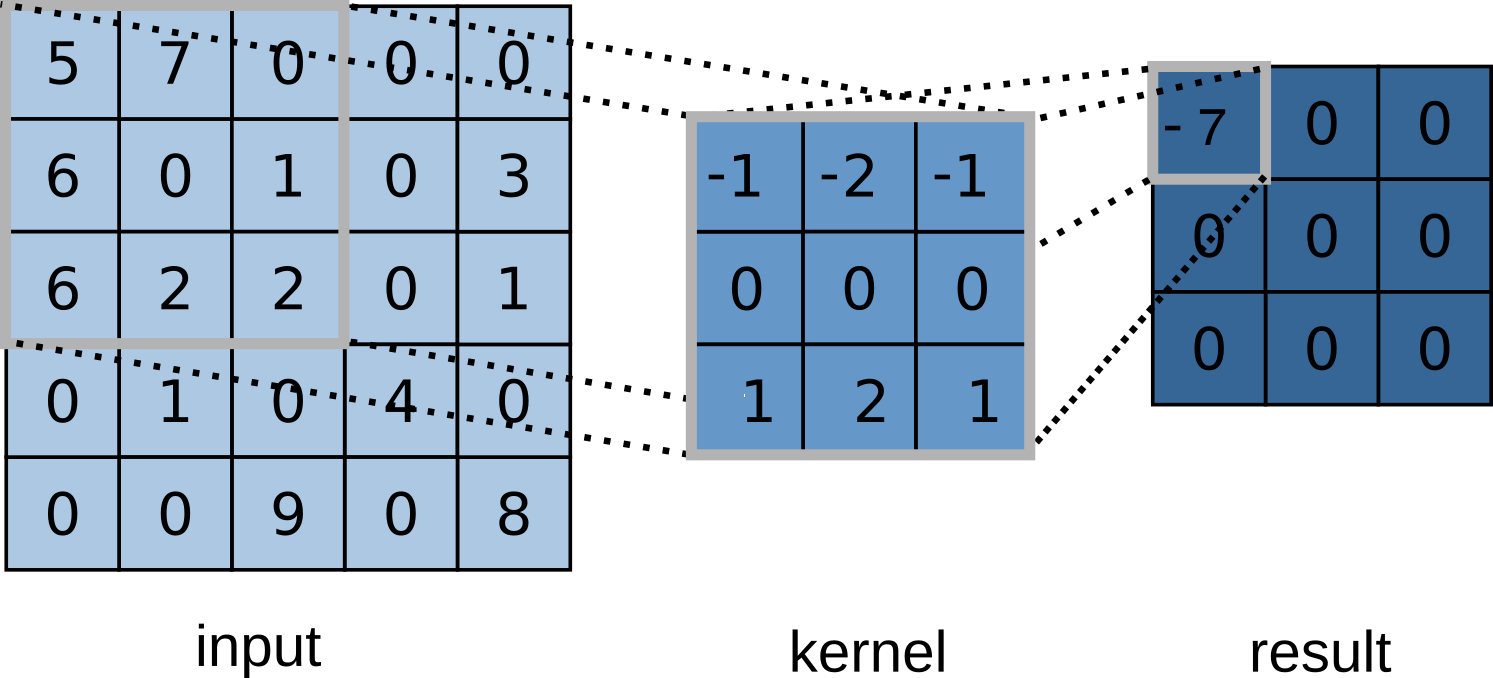
\includegraphics[scale=0.40]{"Part 3 - Learning Systems/Supervised Learning/Deep Learning/images/figure117.png"}
    \caption{Convolution of a 5x5 sized image with a 3x3 sized kernel and its result.}
    \label{fig:figure117}
\end{figure}

In Figure \ref{fig:figure117}, a single matrix $F$ corresponding to an image is being used. In a real world application, this would correspond to a grayscale image. However, most of the time images will be following the RGB (Red, Green Blue) model, where three matrices will be present, each one representing a color channel. These three matrices represent an image in colour. You may also refer to these three 2-dimensional matrices together as a single 3-dimensional matrix. When using RGB images, there will be one kernel for each channel. You may refer to these three kernels together  as a 3-dimensional filter. Using this terminology, applying a 3-dimensional filter to a 3-dimensional image will result in an image represented by a single matrix corresponding to the sum of the three matrices obtained by applying each kernel to its corresponding 2-dimensional matrix. Figure \ref{fig:figure118} depicts an example of convolution for an RGB image. %An important thing to note is that the number of layers in the input filter has to be equal to the number of channels in the image for the convolution operation to be done.

\begin{figure}[h]
    \centering
    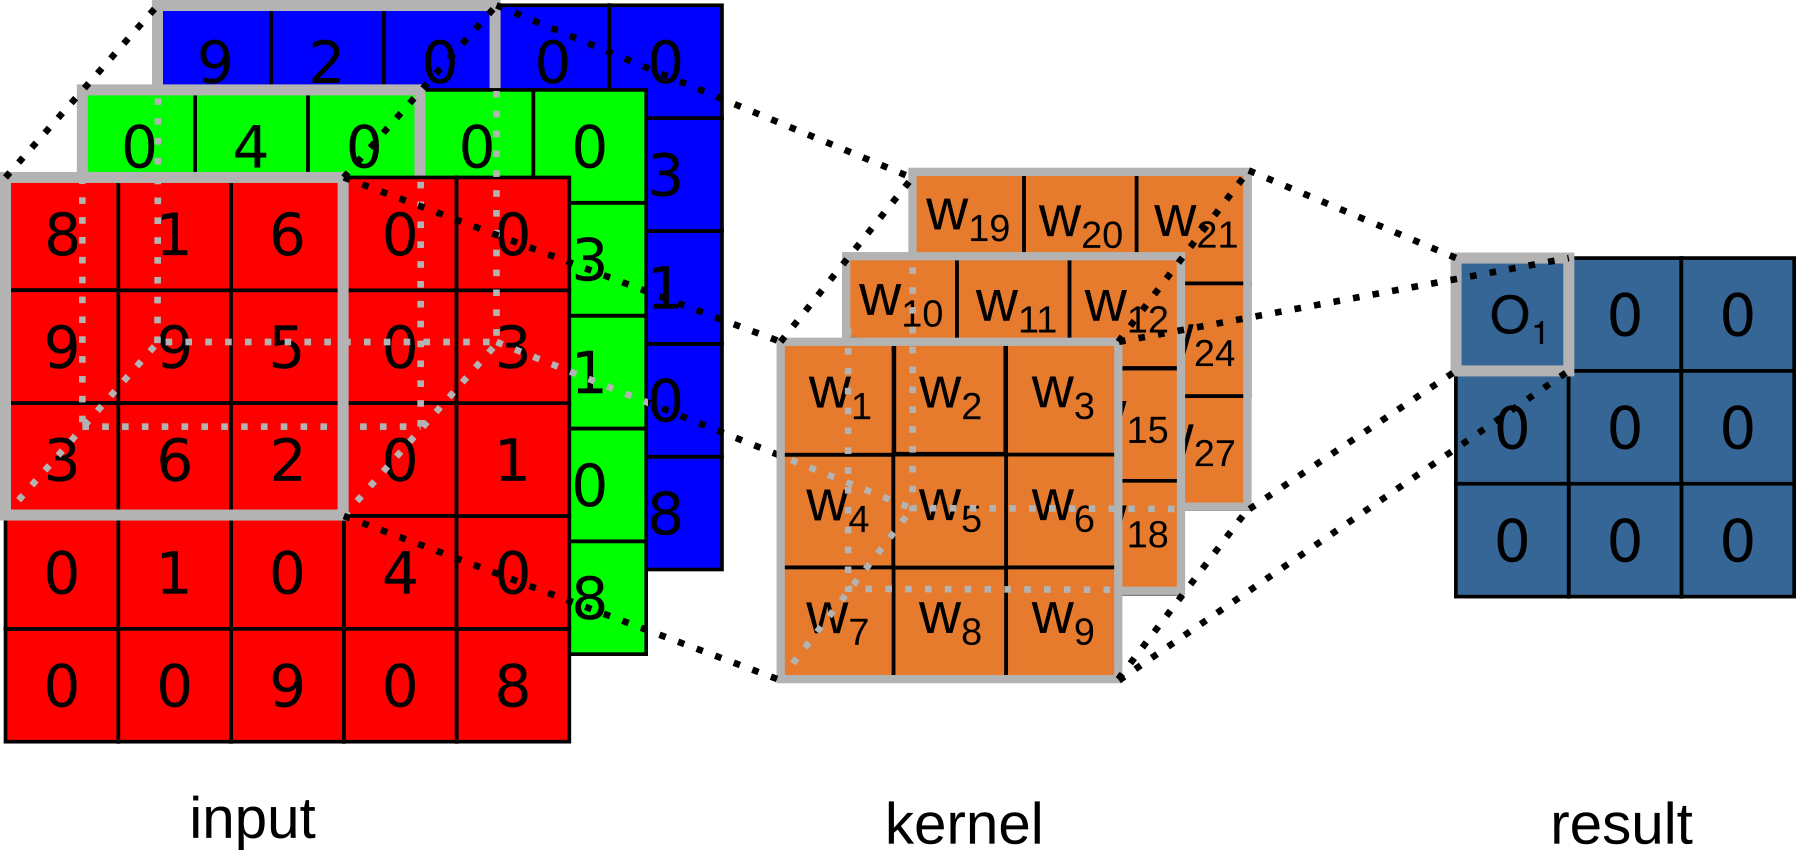
\includegraphics[scale=0.35]{"Part 3 - Learning Systems/Supervised Learning/Deep Learning/images/figure118.png"}
    \caption{Convolution of a 5x5x3 sized image with a 3x3x3 sized kernel and its result.} 
    \label{fig:figure118}
\end{figure}

In addition, one may wish to apply more than one filter to a given image. This will result in multiple images being produced as output. An example of that is given in Figure \ref{fig:figure119}, which depicts a representation of a convolution layer with three filters. For each filter, there is an output matrix and, consequently, as a final result a dataset where the number of depth layers (also known as feature map, illustrated by the three matrices in orange) will correspond to the number of filters applied to the input. This output can then be sent forward on the network, going through more convolutions and having more features extracted.

\begin{figure}[h]
    \centering
    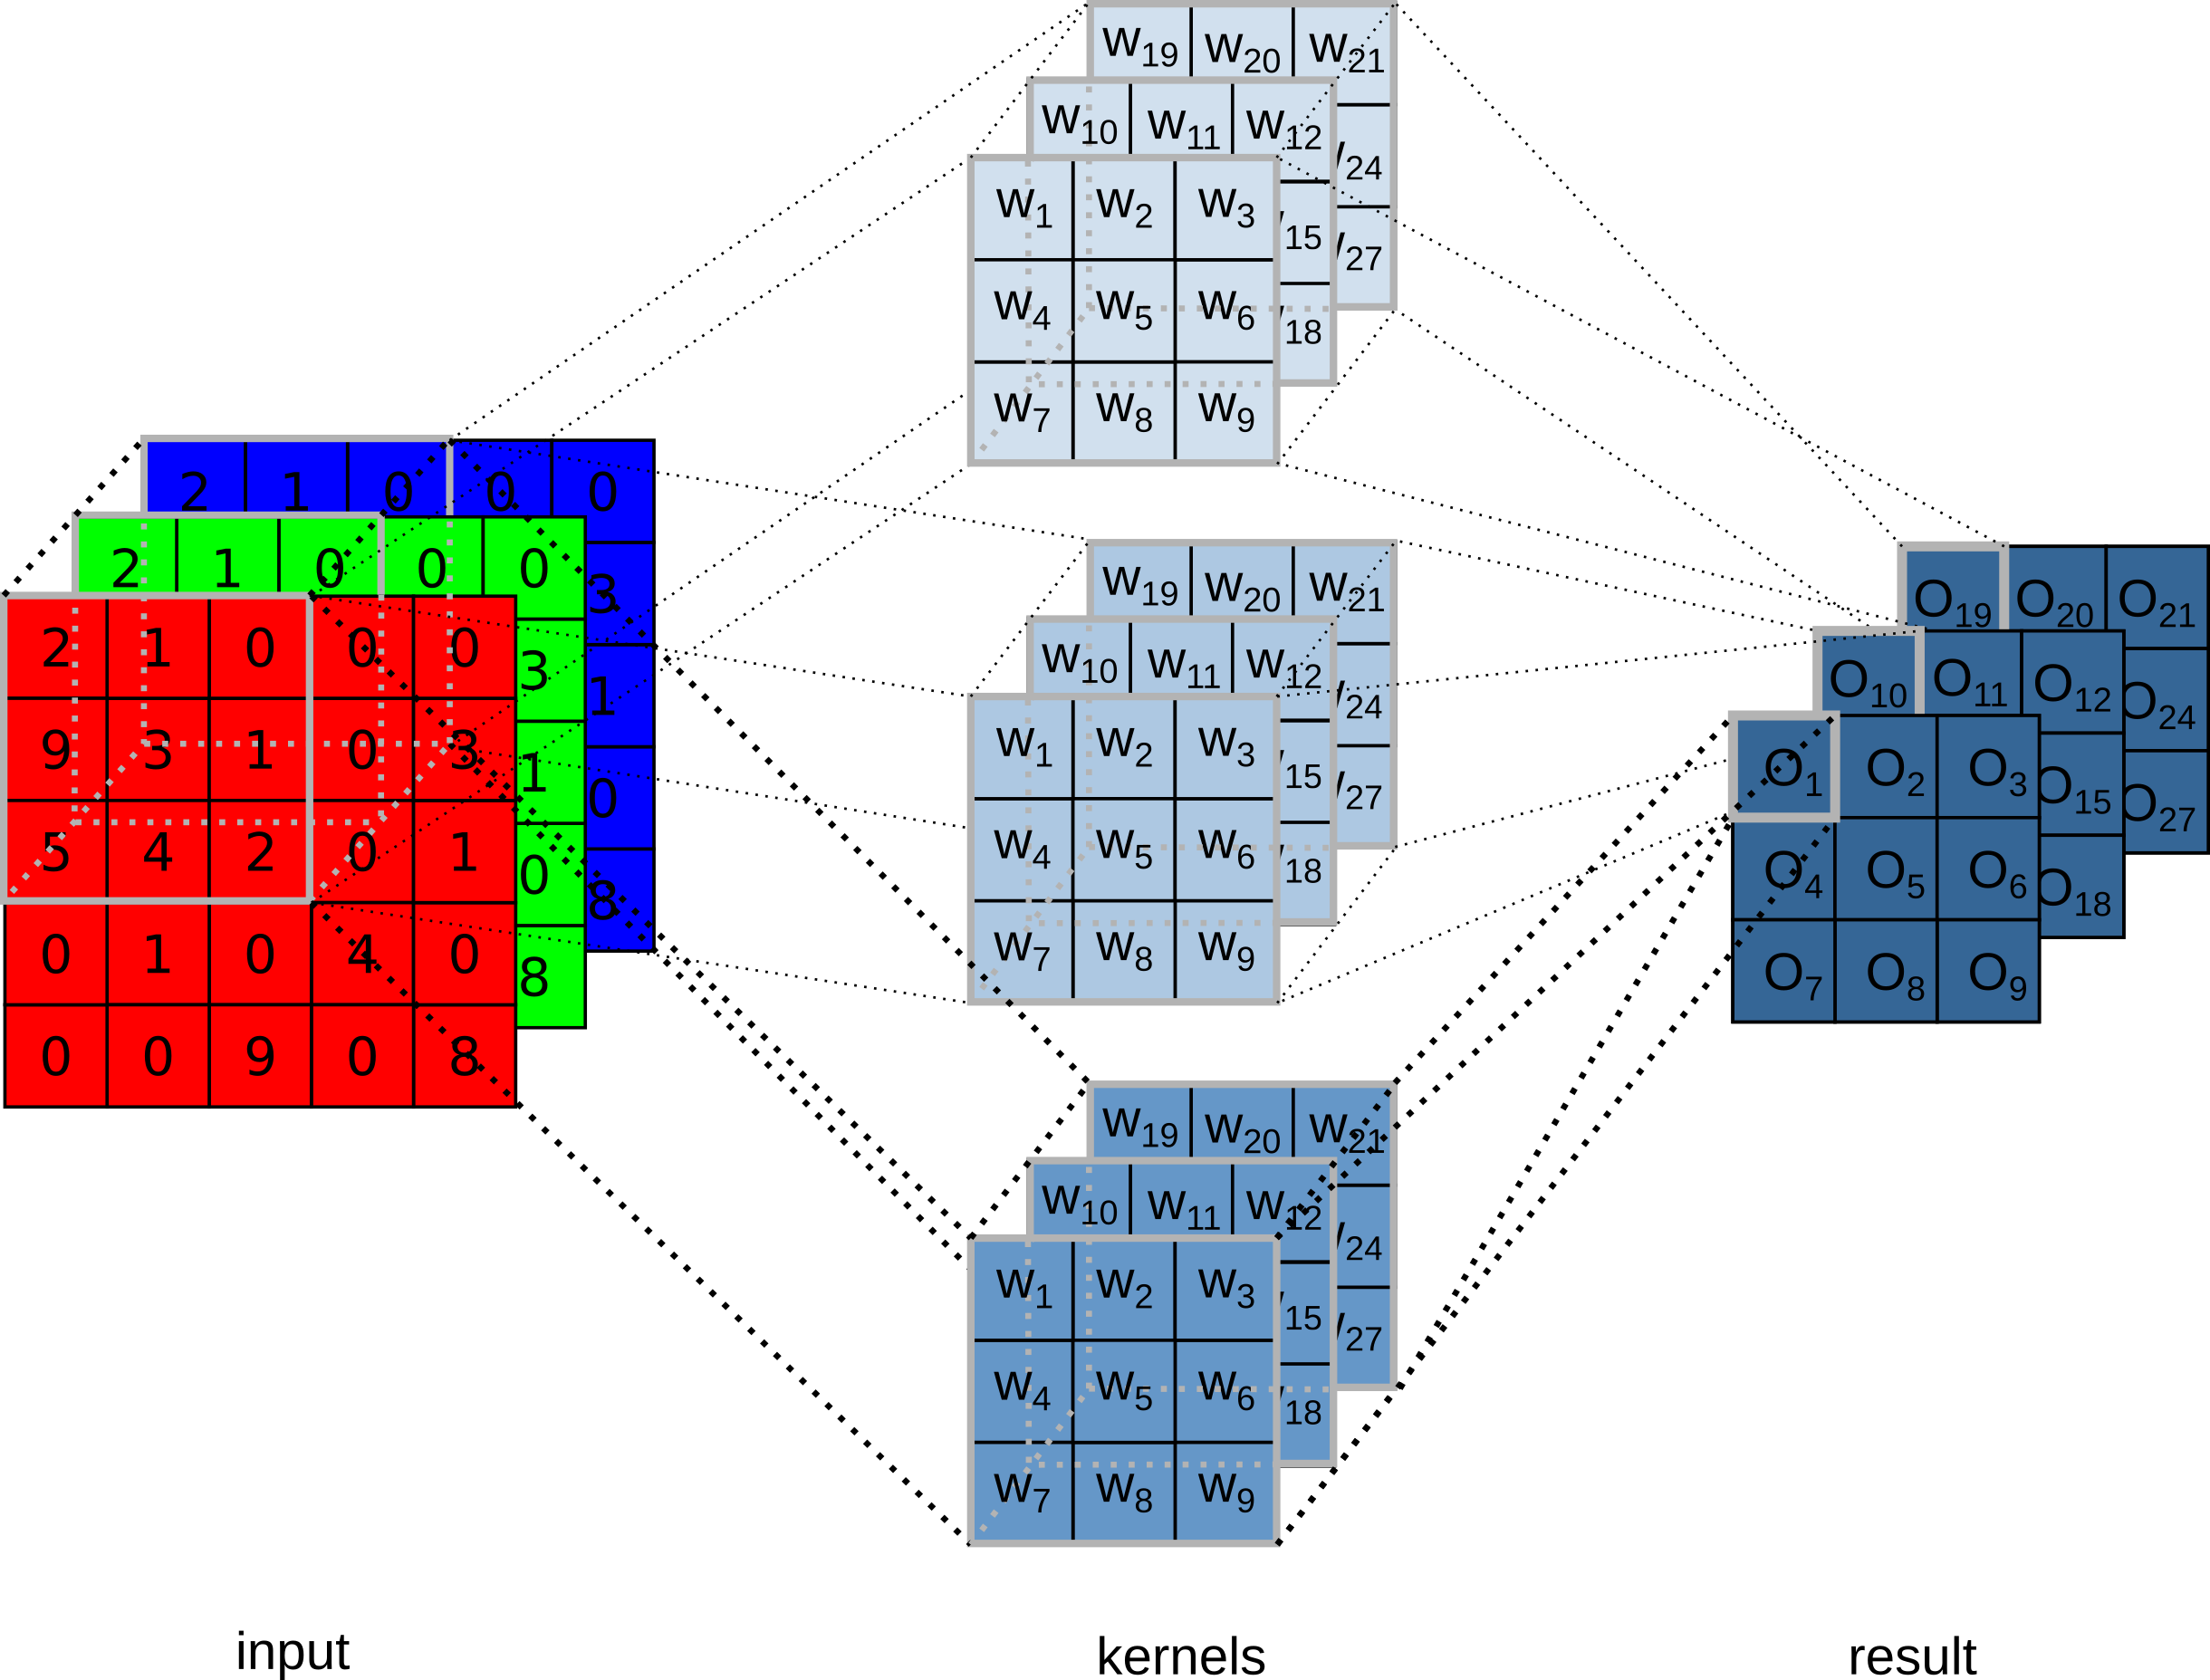
\includegraphics[scale=0.25]{"Part 3 - Learning Systems/Supervised Learning/Deep Learning/images/figure119.png"}
    \caption{Convolution of a 5x5x3 sized image with three 3x3x3 sized kernel and its result.}
    \label{fig:figure119}
\end{figure}

These examples also serve to show us one of the features of convolution that makes it a good choice for working with images, what is called feature sparse iterations (also known as sparse connectivity) \cite{goodfellow2016}. This attribute highlights the fact that each output unit, or pixel, is connected to only a fraction of the input units. For example, in Figure \ref{fig:figure119}, each output pixel is connected to a region of the 75 input pixels, through a 3x3x3 kernel. This is very useful, as our image can have millions of pixels, and by using smaller sized kernels, we will be able to detect small features such as edges, corners, etc \cite{goodfellow2016}. In the convolution layers, the learning process consists in learning the filters. This results in few parameters to learn and store. Conversely, in a simple neural network, as we saw in the MLP chapter, an image at the input means that each pixel would be connected to each neuron in the next layer, thus resulting in an excessively large network.

As mentioned earlier, another important feature of CNNs is the ability to share the parameters to be learned, since the same filter is applied to different regions of the image using the same values. This is unlike a neural network without convolution layers, where we have a matrix with weights that are used for only one connection. The sharing of parameters gives us another feature, which is the invariance to translation, i.e., if we move the position of an object in the input image, its representation will also be moved in the resulting image \cite{goodfellow2016}.

\subsubsection{Padding}

In the convolution examples, Figures \ref{fig:figure117} to \ref{fig:figure119}, we see that as we apply the kernel to the input image, the size of the output image is reduced. In fact, by convolving an image of size $m \times n$ with a kernel of size $k_m \times k_n$ the resulting image will have a height of $m-k_m+1$ and a length of $n-k_n+1$ . This type of convolution, where the resulting image is smaller, is often called ``valid''.
If we want the output image to be the same size as the input image, we have to add more rows and columns to our image, this is known as padding. In this case, we use the formula  $m+2p_m-k_m+1$ and $n+2p_n-k_n+1$ to represent the size of the new dimensions of the image. Here, $p_m$ represents the number of rows to be added to the image, roughly half at the top and half at the bottom of the image. Similarly, $p_n$ represents the number of columns to be added to the image, roughly half at the left and half at the right size of the image. For example, in the previous Figure \ref{fig:figure117}, if the output has to be the same size as the input, we would have to use a padding of $p_m=p_n=1$. So, padding would increase the dimensions of the input image from 5 by 5 to $6+2p_m-3+1$ by $6+2p_n-3+1$, i.e., 6 by 6. Typically, the value of the new pixels added to the image is zero.

\subsubsection{Stride}

The convolution examples we saw earlier used unitary steps, i.e., the kernel is applied by sliding through the pixels of the input image one by one. However, we can also use larger steps, as this reduces the computational cost of performing these steps at intervals. %When we use a stride value greater than one, this will also affect the output size, which will be governed by the following relationship \cite{adrian2017}:
%
%\begin{equation}
%\frac{m+2p-k_m}{s}+1 \  \times \ \frac{n+2p-k_n}{s}+1
%\end{equation}
%
%Where $m$ and $n$ are the image dimensions, $p$ is the padding, $k_m$ and $k_n$ are the kernel dimensions and $s$ is the stride. 
Figure \ref{fig:stride} depicts an example with the steps of a convolution with stride=2 using a kernel of size 3 over an image of size 5 x 5 and no padding.
This clearly has an impact on the resulting output, decreasing its resolution, but in cases where we do not need to extract delicate features this becomes a good option \cite{goodfellow2016}.

\begin{figure}[h]
    \centering
    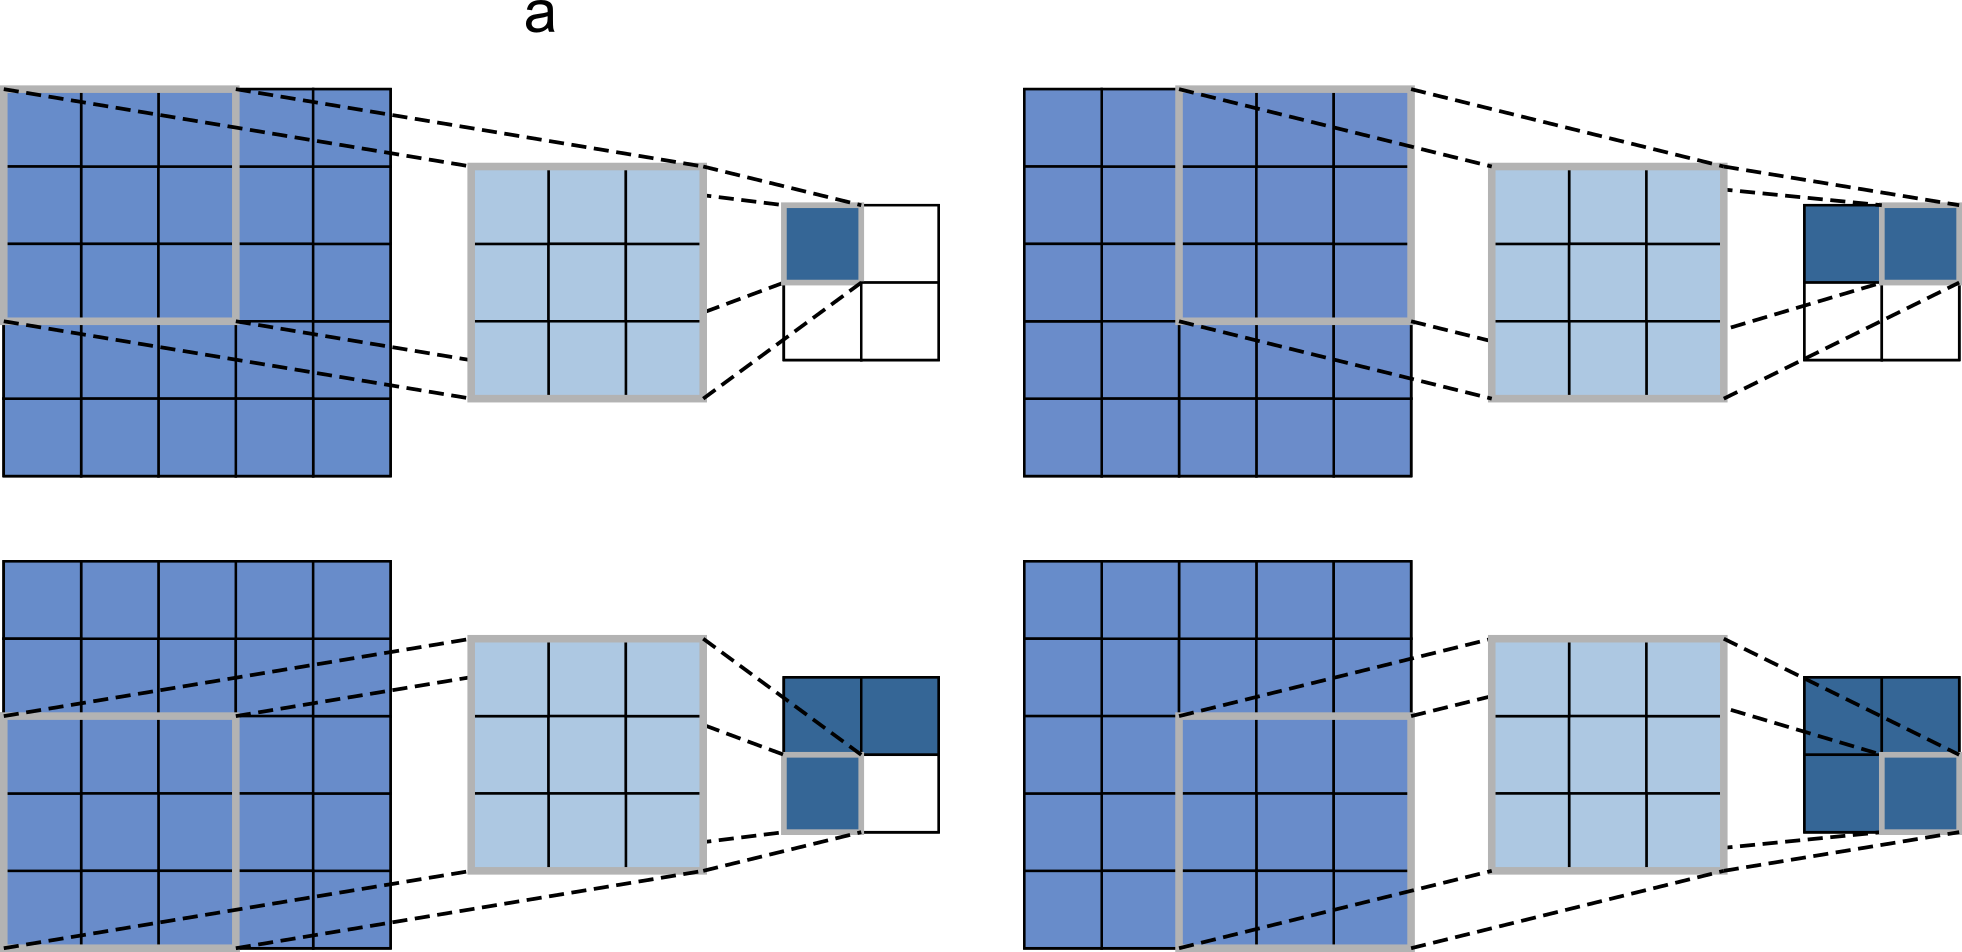
\includegraphics[scale=0.20]{"Part 3 - Learning Systems/Supervised Learning/Deep Learning/images/stride.png"}
    \caption{Example using stride=2.}
    \label{fig:stride}
\end{figure}


\subsection{Pooling Layers}

This is a very important layer, which aims to subsampling the image to reduce its size, and, consequently, reduce the total memory, processing and parameters needed, in addition to curbing the risk of overfitting \cite{geron2019,adrian2017,elgendy2020}.

As in convolution layers each output unit is connected to an input region, we must also take into account the size of the kernel, stride and padding. But, unlike the convolution, the ``kernel'', or, in other words, the region that will connect us to the input, will have no weights -- it will perform only one operation, the most common being the maximum or the average \cite{geron2019}.

Figure \ref{fig:figure121} depicts an example of max pooling, illustrating how it works (Figures \ref{fig:figure121}(a-d)). This example uses a region of 2 x 2 , which is very common \cite{adrian2017}, and stride=1.

\begin{figure}[h]
    \centering
    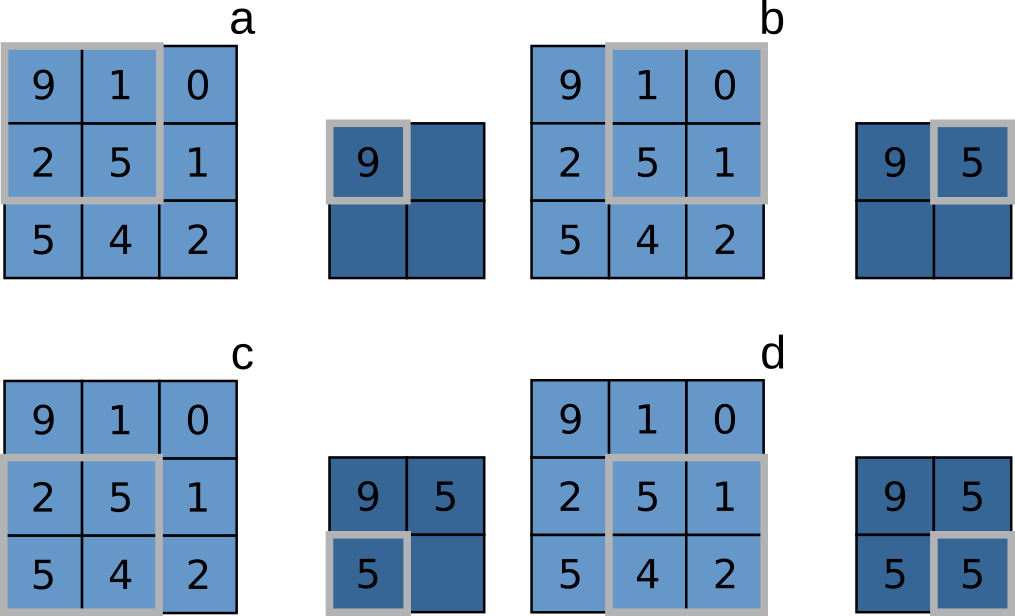
\includegraphics[scale=0.30]{"Part 3 - Learning Systems/Supervised Learning/Deep Learning/images/figure121.png"}
    \caption{Example of max pooling application.}
    \label{fig:figure121}
\end{figure}

Figure \ref{fig:figure122} depicts another example of max pooling, but this time performed with a 3-channel input. We can see that the operation is performed on each input channel of the object, and that its output contains the same number of channels as the input, which is what is typically done in this type of operation \cite{geron2019}.

\begin{figure}[h]
    \centering
    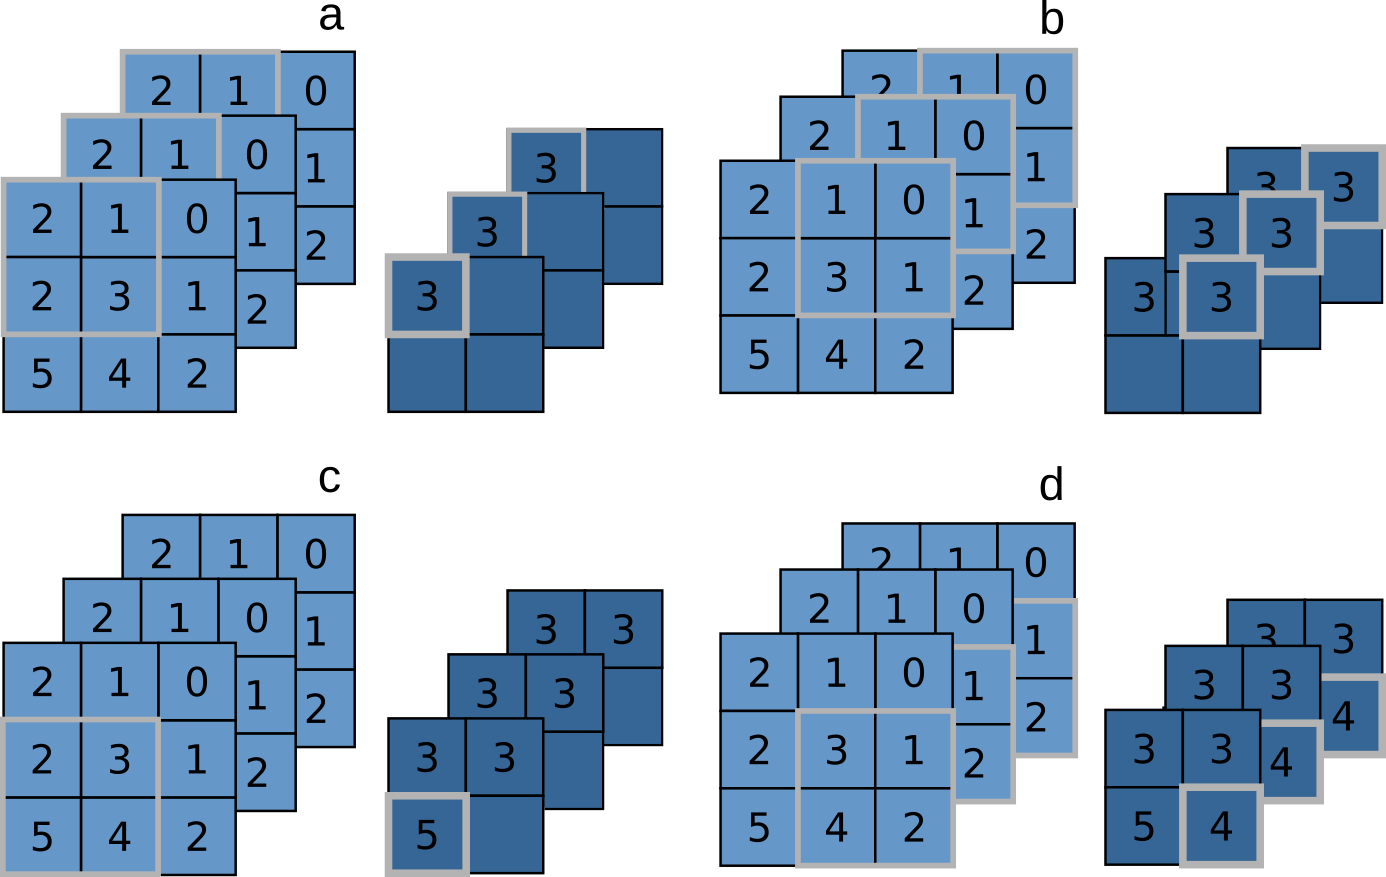
\includegraphics[scale=0.30]{"Part 3 - Learning Systems/Supervised Learning/Deep Learning/images/figure122.png"}
    \caption{Example of max pooling application in an image with more dimensions.}
    \label{fig:figure122}
\end{figure}

Although pooling is a very popular technique, we can find scientific works where their authors preferred not to use pooling to perform subsampling, but to use convolution layers with higher stride and appropriate padding values to achieve dimension reduction \cite{elgendy2020,adrian2017}. This way of working was proposed by Springenberg \cite{springenberg2014striving}, where they demonstrated that even networks without pooling layers can yield good results for some datasets. % such as CIFAR-10 and ImageNet.

\subsection{Fully Connected Layers}

CNNs usually have several convolution layers followed by activation functions, which in turn are followed by pooling layers, and this process decreases the dimensions $m \times n$ and increases the depth of the CNN model, that is, the number of feature maps generated by it \cite{elgendy2020,geron2019}. These feature maps represent the characteristics extracted from the input image, and we need to use this information as features to be given as input to fully connected layers, which are used to map these features to the desired outputs of the neural network. The fully connected layers are basically an MLP \cite{elgendy2020}, where each neuron of a given layer is fully connected to all neurons of the next layer.

Figure \ref{fig:figure124} illustrates fully connected layers. The input vector is composed of the feature maps produced by the layer that immediately precedes the fully connected layers. In this example, the feature map has a size of 7x7x64, that is, we have 64 feature maps of size 7x7. To provide these features as input to the fully connected layer, we have to flatten these feature maps to a vector of dimensions 1x3136, that passes through the network and ends in the Softmax layer, whose neurons have softmax activation functions (see chapter about MLP for activation functions), resulting in the output vector.

\begin{figure}[h]
    \centering
    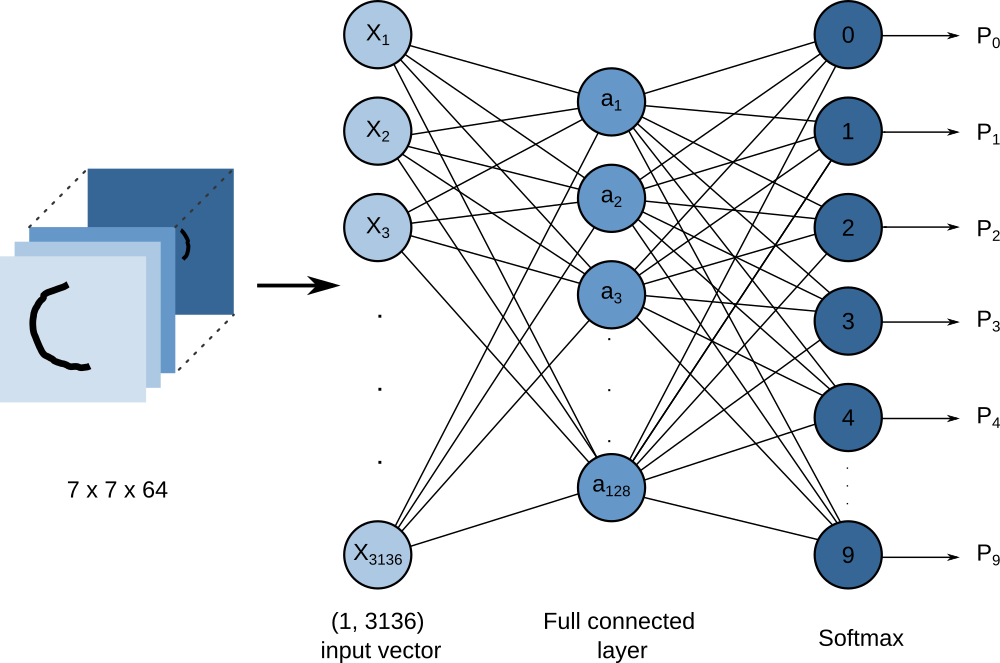
\includegraphics[scale=0.50]{"Part 3 - Learning Systems/Supervised Learning/Deep Learning/images/figure124.png"}
    \caption{Example of fully connected layers application in an image with more dimensions.}
    \label{fig:figure124}
\end{figure}

